\documentclass[conference, a4paper]{IEEEtran}[2015/08/26]
\IEEEoverridecommandlockouts
% The preceding line is only needed to identify funding in the first footnote. If that is unneeded, please comment it out.
%Template version as of 6/27/2024

\usepackage{cite}
\usepackage{amsmath,amssymb,amsfonts}
\usepackage{algorithmic}
\usepackage{graphicx}
\usepackage{textcomp}
\usepackage{xcolor}

\usepackage{float} 
\usepackage{placeins}

\usepackage{colortbl}  % Required for \rowcolor
\usepackage{xcolor}    % Provides additional color definitions

% Digunakan untuk menampilkan pustaka.
\usepackage[square,comma,numbers,sort&compress]{natbib}

% Mengubah format ukuran teks pada natbib.
\renewcommand{\bibfont}{\normalfont\footnotesize}

% Digunakan untuk menyeimbangkan bagian akhir dokumen dengan dua kolom.
\usepackage{balance}

\def\BibTeX{{\rm B\kern-.05em{\sc i\kern-.025em b}\kern-.08em
    T\kern-.1667em\lower.7ex\hbox{E}\kern-.125emX}}
\begin{document}


% \title{AUTONOMOUS VEHICLE NAVIGATION SYSTEM USING MACHINE LEARNING AND GRAPH BASED SLAM
% }
% \title{AUTONOMOUS VEHICLE NAVIGATION FOR HEAVY INDUSTRIAL TRANSPORT WITH HIGH ACCURACY AND PRECISION POSE USING GRAPH-BASED SLAM AND REAL-TIME MACHINE LEARNING}

\title{HYBRID NAVIGATION SYSTEM FOR INDUSTRIAL AUTONOMOUS VEHICLE USING EXTENDED RTAB-MAP AND REDUCED FAST-SCNN}

\author{\IEEEauthorblockN{Azzam Wildan Maulana}
\IEEEauthorblockA{\textit{Department of Electrical Engineering} \\
Institut Teknologi Sepuluh Nopember\\
Surabaya, Indonesia 60111 \\
6022241101@student.its.ac.id}
\and
\IEEEauthorblockN{Rudy Dikairono}
\IEEEauthorblockA{\textit{Department of Electrical Engineering}\\
Institut Teknologi Sepuluh Nopember\\
Surabaya, Indonesia 60111 \\
rudydikairono@its.ac.id}
\and
\IEEEauthorblockN{Ahmad Zaini}
\IEEEauthorblockA{\textit{Department of Electrical Engineering}\\
\textit{Department of Computer Engineering}\\
% Faculty of Intelligent Electrical and Informatics Technology\\
Institut Teknologi Sepuluh Nopember\\
Surabaya, Indonesia 60111 \\
zaini@its.ac.id}
\and
\IEEEauthorblockN{Moh Ismarintan Zazuli}
\IEEEauthorblockA{\textit{Department of Electrical Automation Engineering} \\
Institut Teknologi Sepuluh Nopember\\
Surabaya, Indonesia 60111 \\
ismarintan@its.ac.id}
\and
\IEEEauthorblockN{Muhtadin}
\IEEEauthorblockA{\textit{Department of Computer Engineering} \\
Institut Teknologi Sepuluh Nopember\\
Surabaya, Indonesia 60111 \\
muhtadin@ee.its.ac.id}
\and
\IEEEauthorblockN{Mauridhi Hery Purnomo}
\IEEEauthorblockA{\textit{Department of Electrical Engineering} \\
\textit{Department of Computer Engineering}\\
% \textit{Faculty of Intelligent Electrical and Informatics Technolog} \\
Institut Teknologi Sepuluh Nopember\\
Surabaya, Indonesia 60111 \\
hery@ee.its.ac.id}
}

\maketitle

% \begin{abstract}
% 	This research develops a dual-layer navigation system for industrial autonomous vehicles. The first layer, an Extended RTAB-Map, performs global navigation and mapping. The second, a Reduced Fast-SCNN, handles local perception for lane detection. The Extended RTAB-Map introduces a skip connection from wheels and IMU to pose fusion. The Reduced Fast-SCNN decreases convolutional channels and replaces pyramid pooling with average pooling. Experiments show an increase in pose update rate from 1~Hz to 50~Hz with centimeter-level accuracy (error $<5$~cm). The Reduced Fast-SCNN achieves real-time CPU-only inference below 10~ms.
% 	\end{abstract}

% \begin{abstract}
% 	Navigation system is a crucial part of autonomous vehicle, especially in industrial environment where safety and efficiency are paramount. It is typically divided into two main parts. The first part is global navigation system. The second part is local navigation system. Many of the existing indoor global navigation system used Visual SLAM. However, most of them have low update rate (around 1 Hz) and heavily rely on lighting condition and visual features. To overcome these limitations, we proposed an Extended RTAB-Map by utilizing RTAB-Map and using a skip connection from wheels and IMU odometry to pose fusion. In part of local navigation system, there are many existing deep learning-based semantic segmentation models such as Fast-SCNN and D-Fast-SCNN. However, they are still too heavy to run on CPU-only. Running Fast-SCNN on Intel i5 11th Gen CPU with 12 GB RAM and no dedicated GPU only achieved around 29.5 ms inference time. To meet the real-time requirement in industrial environment, we proposed a Reduced Fast-SCNN by reducing convolutional channels and replacing pyramid pooling with average pooling. The proposed Reduced Fast-SCNN achieved around 7.63 ms inference time on the same hardware platform. By using the Extended RTAB-Map and Reduced Fast-SCNN, we developed a CPU-only navigation system that achieved high-frequency (50 Hz) and high-accuracy (error $<5$ cm) pose estimation together with real-time lane detection (inference time $<10$ ms). 
% \end{abstract}

\begin{abstract}
	The navigation system is a crucial component of an autonomous vehicle, especially in industrial environments where safety and efficiency are paramount. It is typically divided into two main parts: the global navigation system and the local navigation system. Most existing indoor global navigation systems rely on visual SLAM, which suffers from low update rates (around 1~Hz) and strong dependence on lighting conditions and visual features. To address these limitations, this research proposes an Extended RTAB-Map that integrates wheels and IMU from wheel encoders and IMU data through a skip connection to the pose fusion stage. For the local navigation system, many deep learning-based semantic segmentation models such as Fast-SCNN and D-Fast-SCNN remain too computationally heavy for CPU-only operation. Running Fast-SCNN on 2.40 Ghz quadcore CPU with 16 GB RAM and without dedicated GPU yields an average inference time of 29.5~ms. To meet real-time industrial requirements, we developed a Reduced Fast-SCNN by lowering convolutional channels and replacing pyramid pooling with average pooling. The proposed Reduced Fast-SCNN achieves 7.63~ms inference on the same hardware. Combining the Extended RTAB-Map and Reduced Fast-SCNN results in a CPU-only navigation system capable of high-frequency (50~Hz) and high-accuracy (error~$<5$~cm) pose estimation with real-time lane detection (inference~$<10$~ms).
	\end{abstract}

\begin{IEEEkeywords}
	navigation system, RTAB-Map, Fast-SCNN, RTAB-Map SLAM, machine learning, lane detection, autonomous vehicle 
\end{IEEEkeywords}


\section{Introduction}
Autonomous vehicles are increasingly vital in industrial logistics, offering improvements in safety, efficiency, and operational precision. Industrial plants often require continuous material transport in constrained and hazardous environments, where human operators are prone to fatigue and error. As reported in \cite{ref_sleep}, night-shift workers are particularly susceptible to micro-sleep episodes lasting one or two seconds, which can result in serious accidents. To mitigate these risks, autonomous vehicles can replace or assist human-operated systems, ensuring continuous and safe material handling.

\par
An autonomous navigation system generally consists of two main components: the global navigation system for estimating pose of vehicle, and the local navigation system for controlling vehicle motion inside vehicle lookahead distance. The global system requires both accuracy and high update rates to maintain control stability. In this research, we extend the Real-Time Appearance-Based Mapping (RTAB-Map) algorithm \cite{ref_rtabmap} to achieve higher update rate and accuracy. The default RTAB-Map provides a limited update rate (around 1~Hz) and is heavily dependent on visual odometry, which suffers under lighting variations or occlusions \cite{ref_vslam}. To overcome these limitations, an \textit{Extended RTAB-Map} is proposed by introducing a skip connection from wheels and IMU odometry to pose fusion. Odometry data from wheels and IMU sensors are combined with RTAB-Map’s corrected pose using a Kalman Filter \cite{ref_mas_marin}, improving both update frequency and pose accuracy.

\par
For local navigation, lane or drivable-area detection is essential for maintaining safe motion. Deep learning-based semantic segmentation models like Fast-SCNN \cite{ref_fast_scnn} are efficient but still computationally heavy for CPU-only systems. Although D-Fast-SCNN \cite{ref_dfast_scnn} improves accuracy using dilation, it increases inference time. To meet real-time industrial demands, we design a \textit{Reduced Fast-SCNN} by lowering convolutional channels and replacing pyramid pooling with average pooling, achieving sub-10~ms inference on CPU. The output segmentation provides a confidence level used to adjust vehicle speed and steering dynamically. By integrating the Extended RTAB-Map and Reduced Fast-SCNN, this research delivers a high-frequency, CPU-efficient, and centimeter-accurate navigation system suitable for industrial autonomous vehicles.

% =========================================================================================================

\section{Methodology}
The methodology of this research is divided into three main parts. The first part discusses the architecture of the Extended RTAB-Map. The second part presents the network design of the Reduced Fast-SCNN. The final part explains the integration of the Extended RTAB-Map and Reduced Fast-SCNN into a unified navigation system for autonomous industrial vehicles.

\subsection{Extended RTAB-Map for Global Navigation System}
\begin{figure}[H]
	\centering
	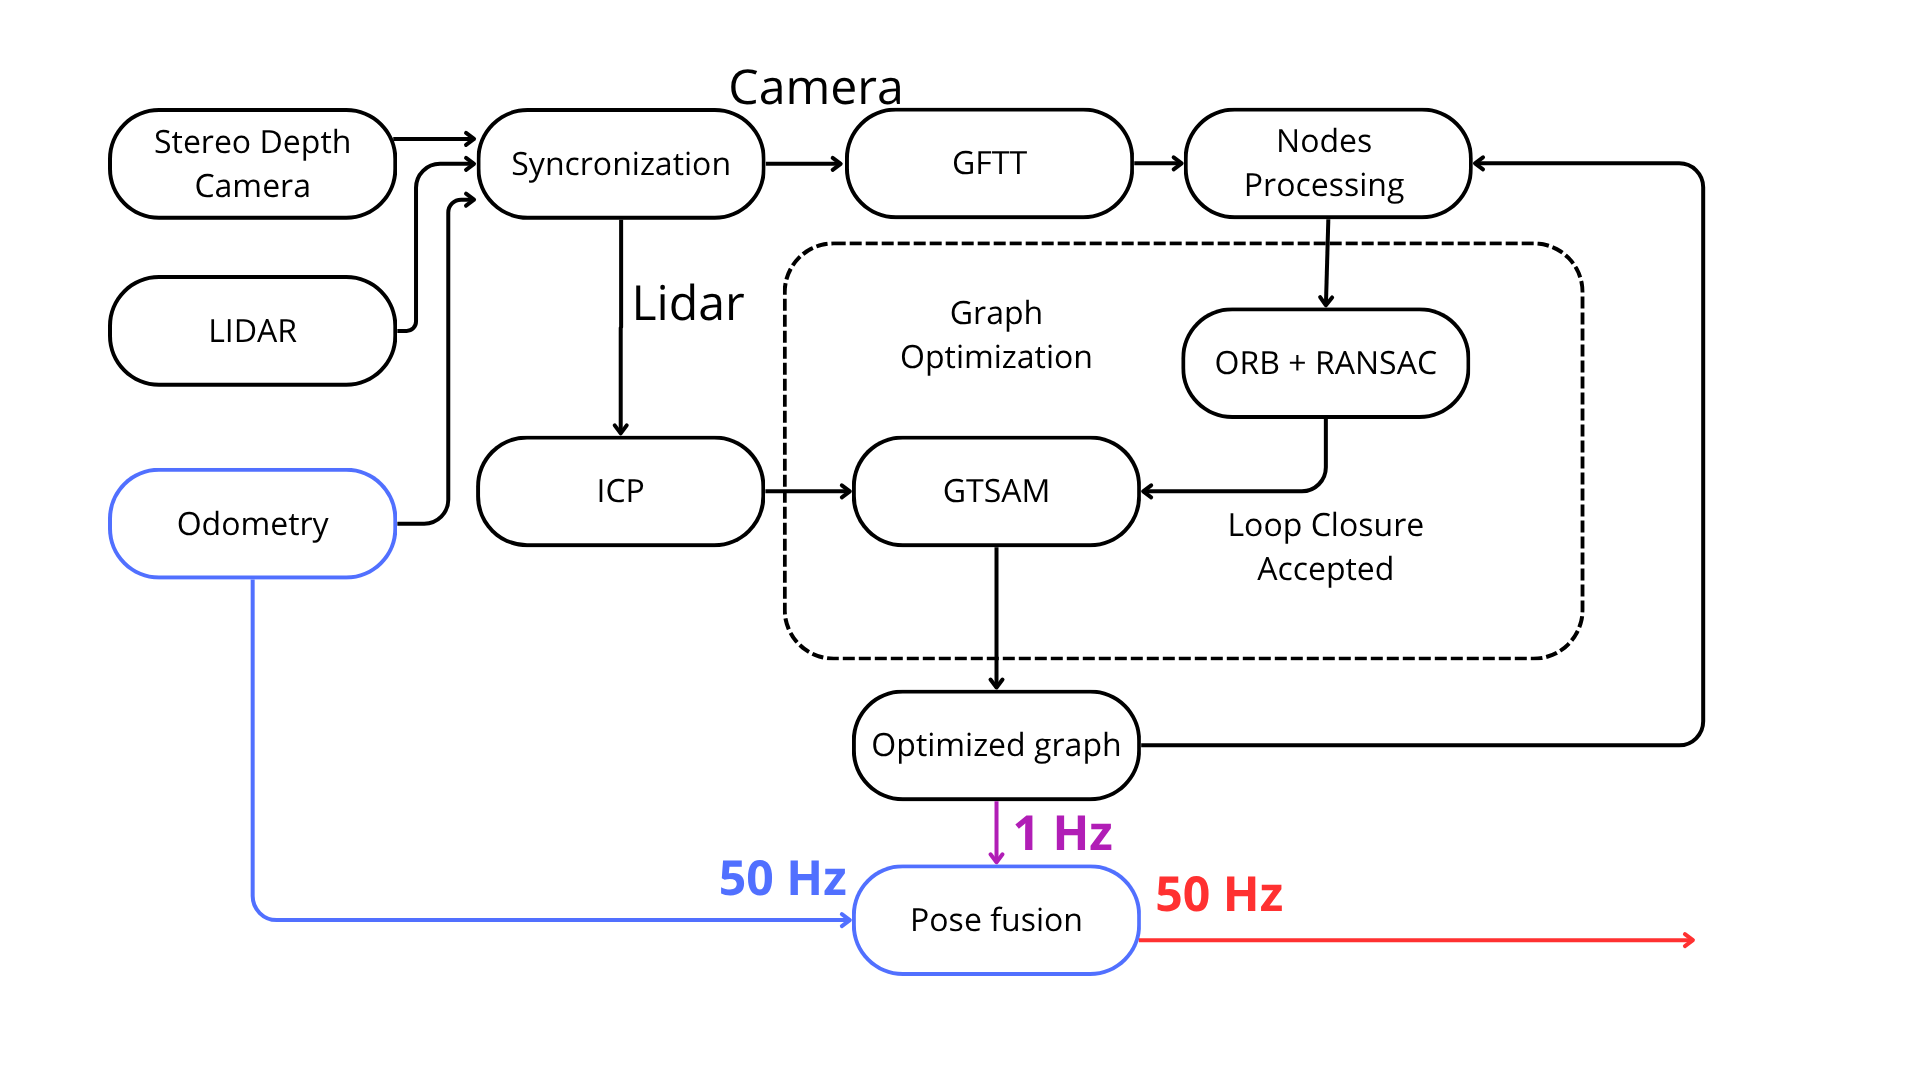
\includegraphics[width=\linewidth]{../konten/slam_fix_iki.png}
	\caption{Block diagram of Extended RTAB-Map architecture. The blue line indicates the skip connection from wheels and IMU odometry to pose fusion.}
	\label{fig:slam_system}
\end{figure}

\subsubsection{Odometry Calculation from Wheels and IMU}
The most important step is to calculate the wheels and IMU using encoder speed and IMU data. The relationship can be expressed as follows:

\begin{equation}
	\begin{bmatrix}
	v_x \\
	v_y \\
	v_\theta
	\end{bmatrix}
	=
	\dfrac{1}{\Delta t}
	\begin{bmatrix}
	\text{encoder\_to\_meter}\,\text{encoder\_speed}\,\cos\theta \\
	\text{encoder\_to\_meter}\,\text{encoder\_speed}\,\sin\theta \\
	\text{current\_IMUyaw}-\text{previous\_IMUyaw}
	\end{bmatrix}
	\label{eq:velocity_matrix_explicit}
\end{equation}

Here, $v_x$ represents the linear velocity in the x-direction, $v_y$ is the linear velocity in the y-direction, and $v_\theta$ is the angular velocity around the z-axis. The term $\Delta t$ denotes the time difference between the current and previous readings (20~ms). The variable $\text{encoder\_to\_meter}$ is a conversion factor from encoder speed (in rpm) to meters per second. $\text{encoder\_speed}$ refers to the encoder output, $\theta$ is the yaw angle from the IMU in radians, while $\text{current\_IMUyaw}$ and $\text{previous\_IMUyaw}$ denote the consecutive IMU yaw readings in degrees.

\subsubsection{Utilize RTAB-Map Synchronization Strategy}
To handle multiple sensors with multiple update frequency too, we utilizing the RTAB-Map synchronization strategy. By default, RTAB-Map use exact sync strategy that require all the sensor update their data at a same time. That strategy so hard to be implemented because each sensor operate independently with difference update frequency. So we change the synchronization strategy to approximate sync. This strategy allow each sensor to not have exactly same timestamp, but still close enough. 

\subsubsection{Utilize RTAB-Map Loop Closure Detection}
The second optimization of RTAB-Map involves the use of the GFTT (Good Features to Track) algorithm as an image feature detector. As demonstrated in \cite{ref_image_matching}, GFTT provides a fast yet reliable feature extraction performance suitable for real-time applications. The third improvement applies the combination of ORB (Oriented FAST and Rotated BRIEF) and RANSAC (Random Sample Consensus) for feature matching. ORB provides a computationally efficient descriptor while maintaining robustness, and RANSAC filters out outliers from matched keypoints \cite{ref_orb_ransac}. The output of this step is a loop-closure hypothesis, which indicates that the robot has revisited a previously mapped location. This hypothesis is used to refine and optimize the pose graph.

\subsubsection{Utilize GTSAM Constraint}
The fourth enhancement in RTAB-Map involves applying the ICP (Iterative Closest Point) algorithm to establish constraints between the nodes. ICP is utilized to compute the relative pose and covariance between two adjacent nodes \cite{ref_icp}. This algorithm is selected because 2D LiDAR provide higher geometric accuracy compared to depth information from cameras \cite{ref_lidarvscamera}.

\par
The fifth stage involves full graph optimization using all nodes and edges. When a valid loop-closure hypothesis is detected, the corrected pose and covariance are calculated based on the ICP constraint. These values are then used to optimize the entire pose graph through nonlinear optimization using the GTSAM library \cite{ref_gtsam}. This optimization reduces accumulated drift and improves global map consistency.

\subsubsection{Introduction of Skip Connection from Wheels and IMU to Pose Fusion}
Despite these improvements, the standard RTAB-Map implementation yields an average pose update rate of only 1~Hz when tested on 2.40 Ghz quadcore CPU with 16 GB RAM and without dedicated GPU. To increase the update rate, we introduce a skip connection from the wheels and IMU to the pose fusion module (indicated by the blue line in Fig.~\ref{fig:slam_system}). The pose fusion employs a Kalman Filter to combine the corrected pose and covariance from RTAB-Map with the odometry-based pose and covariance from the hardware sensors. The wheels and IMU, calculated from Eq.~\ref{eq:velocity_matrix_explicit}, serves as the velocity model in the Kalman Filter, while the RTAB-Map output acts as the measurement model.

\subsubsection{Fusion Strategy}
The fusion strategy begins by assigning a low covariance value (around 0.01) to the wheels and IMU odometry, prioritizing responsiveness during the vehicle’s initial motion. As the system detects more loop closures, the covariance of the RTAB-Map corrected pose gradually decreases, allowing it to dominate the fusion process. Consequently, the final pose estimation becomes both accurate and smooth over time. The use of the Kalman Filter not only improves pose accuracy but also minimizes abrupt transitions during map corrections. The resulting fused pose achieves a 50~Hz update rate on the same hardware setup, with centimeter-level precision suitable for real-time navigation.

\subsection{Reduced Fast-SCNN for Local Navigation System}
\begin{figure}[H]
	\centering
	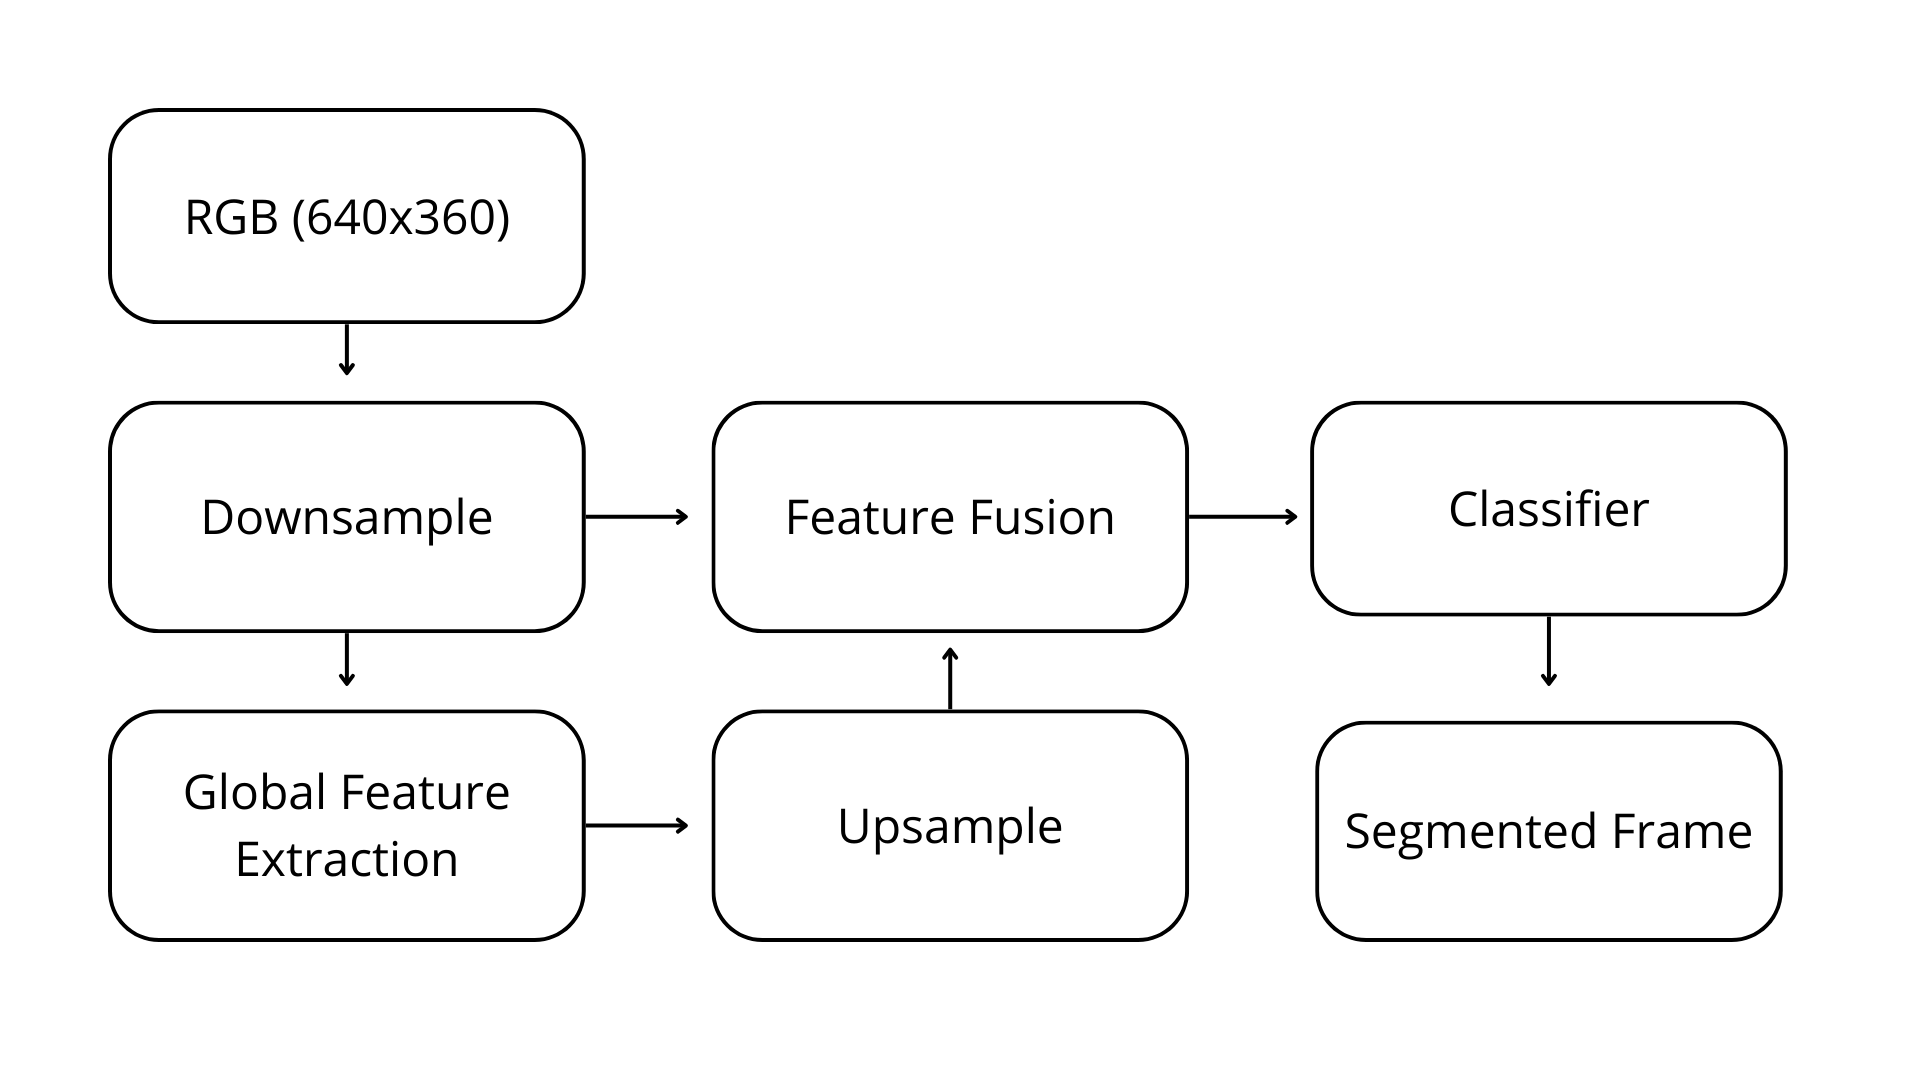
\includegraphics[width=\linewidth]{../konten/ml_sys.png}
	\caption{Block diagram of the Reduced Fast-SCNN architecture.}
	\label{fig:ml_system}
\end{figure}

Building upon the original Fast-SCNN architecture \cite{ref_fast_scnn}, we developed a modified version specifically optimized for lane detection in industrial settings. The original Fast-SCNN was designed for high-speed semantic segmentation on mobile devices; however, in our application, the focus is shifted from segmentation accuracy toward achieving real-time inference on limited computing hardware. The overall structure of the Reduced Fast-SCNN is shown in Fig.~\ref{fig:ml_system}.

\subsubsection{Downsampling}
The Reduced Fast-SCNN begins with a downsampling stage that reduces the input image to a fixed resolution of 360$\times$640 pixels (width $\times$ height). To further reduce computational complexity, the number of convolutional channels is decreased. While the original Fast-SCNN employs 64 channels after downsampling, our modified version uses only 32 channels. This reduction effectively lowers the processing load, with a marginal trade-off in segmentation precision—an acceptable compromise for static and structured industrial environments.

\subsubsection{Global Feature Extraction}
Following the same principle, the global feature extraction stage also reduces the number of channels. In the original architecture, this stage uses 128 channels, whereas in the Reduced Fast-SCNN it is limited to 64 channels. Additionally, the pyramid pooling module is replaced with a lightweight average pooling layer. Compared to pyramid pooling, average pooling simplifies the computation and improves inference speed, making it more suitable for CPU-only real-time operation.

\subsubsection{Upsampling, Feature Fusion, and Classification}
The upsampling, feature fusion, and classification stages retain the core structure of the original Fast-SCNN but operate with fewer convolutional channels. The final output of the Reduced Fast-SCNN is a binary segmentation mask representing two classes: lane and non-lane regions. This segmentation output is later utilized to compute a confidence level that influences the vehicle’s navigation decisions, particularly in adjusting steering and velocity control.

\subsection{Integration of Both Systems}
\begin{figure}[H]
	\centering
	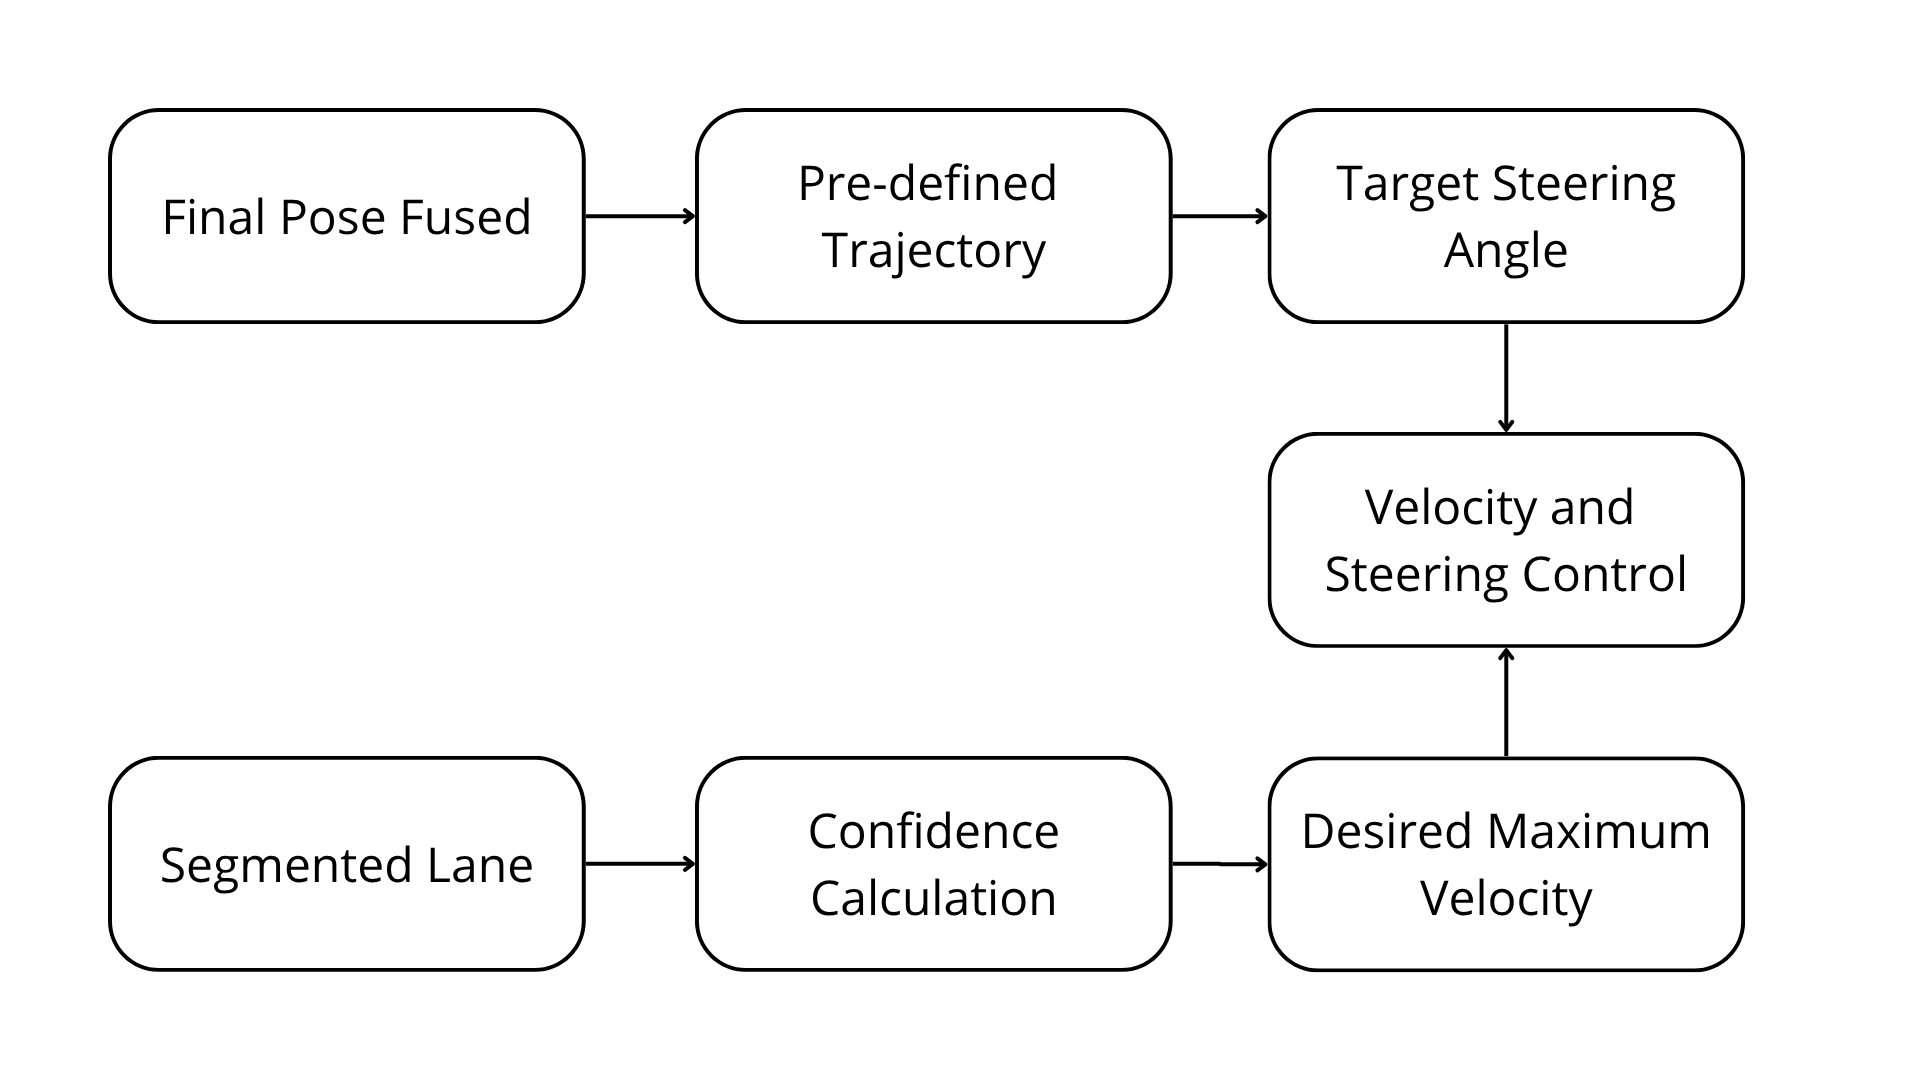
\includegraphics[width=\linewidth]{../konten/hahhhh.png}
	\caption{Integration of the Extended RTAB-Map and Reduced Fast-SCNN for the navigation system.}
	\label{fig:nav_new_system}
\end{figure}

Figure~\ref{fig:nav_new_system} illustrates the integrated navigation framework combining the Extended RTAB-Map for global localization and the Reduced Fast-SCNN for local perception. The navigation controller computes the desired heading angle to the next waypoint as:

\begin{equation}
	\theta_{\text{direction}} = \tan^{-1}\!\left(\frac{y_{\text{wp}} - y_{\text{position}}}{x_{\text{wp}} - x_{\text{position}}}\right) - \theta_{\text{orientation}}
	\label{eq:waypoint_angle}
\end{equation}

where $(x_{\text{wp}}, y_{\text{wp}})$ and $(x_{\text{position}}, y_{\text{position}})$ denote the waypoint and current vehicle positions, respectively, and $\theta_{\text{orientation}}$ is the current heading. Using the Bicycle Model~\cite{rajamani2011vehicle}, the target steering angle is:

\begin{equation}
	\delta_{\text{target}} = \tan^{-1}\!\left( \frac{2L \sin(\theta_{\text{direction}})}{D_{\text{lookahead}}} \right)
	\label{eq:bicycle_model_full}
\end{equation}

where $L$ is the wheelbase and $D_{\text{lookahead}}$ the lookahead distance.

\par
The confidence level from lane segmentation is defined as:

\begin{equation}
	\text{normal} = \frac{\text{area of lane}}{\text{area of ROI}}
	\label{eq:confidence_level}
\end{equation}

and used to modulate the target speed:

\begin{equation}
	v_{\text{target\_max}} = v_{\text{max}} \cdot \text{normal}^2
	\label{eq:confidence_speed}
\end{equation}

A first-order low-pass filter ensures smooth velocity transitions:

\begin{equation}
	v_{\text{target}} = \alpha v_{\text{target\_max}} + (1-\alpha)v_{\text{target}}
	\label{eq:low_pass_filter}
\end{equation}

where $\alpha = 0.055$. The resulting $v_{\text{target}}$ and $\delta_{\text{target}}$ are passed to the low-level controller for real-time execution. This integrated approach achieves high-frequency localization and stable motion control on CPU-only hardware.

The $\theta_{\text{target}}$ of steering angle and $v_{\text{target}}$ of velocity are sent to the low-level control layer to be executed in real time. By combining these two subsystems, the navigation system achieves real-time perception and high-frequency localization, enabling stable and accurate motion control even on limited hardware resources.

% =========================================================================================================

\section{Results and Discussion} 
This section presents the experimental results obtained from the proposed navigation system. The evaluation focuses on three key aspects: (1) the accuracy of pose estimation with and without the Extended RTAB-Map, (2) the comparison of update rates between the default RTAB-Map and the Extended RTAB-Map, and (3) the inference performance comparison between the original Fast-SCNN and the proposed Reduced Fast-SCNN. All experiments were conducted on 2.40 Ghz quadcore CPU with 16 GB RAM and without dedicated GPU.

\subsection{Wheels and IMU Odometry Only vs. Extended RTAB-Map} 
The first experiment compared the pose estimation accuracy between the wheels and IMU-only approach and the Extended RTAB-Map. The quantitative results are shown in Table~\ref{tab:pose_estimation}.

\begin{table}[H]
	\centering
	\caption{Pose Estimation Result Using Wheels and IMU Odometry Only}
	\label{tab:pose_estimation}
	\begin{tabular}{|c|c|c|c|}
		\hline
		\textbf{Lap-} & \textbf{X (m)} & \textbf{Y (m)} & \textbf{Error (m)} \\ \hline
		1 & 0.28 & 0.39 & 0.48 \\ \hline
		2 & 0.30 & 0.43 & 0.52 \\ \hline
		3 & 0.24 & 0.49 & 0.55 \\ \hline
		4 & 0.18 & 0.32 & 0.37 \\ \hline
		5 & 0.37 & 0.41 & 0.55 \\ \hline
		\multicolumn{3}{|c|}{\textbf{Average Error}} & 0.494 \\ \hline
	\end{tabular}
\end{table}

In Table~\ref{tab:pose_estimation}, Lap- represents the lap number, while X (m) and Y (m) denote the final position of the vehicle (in meters) after traveling 500~meters. The Error (m) column shows the deviation of the estimated pose from the ground truth, which was defined as $(x=0, y=0)$. The average error of 0.494~m (49.4~cm) indicates that wheels and IMU alone produces significant drift over time, rendering it unsuitable for precise autonomous navigation. Therefore, pose estimation improvement using the Extended RTAB-Map is essential.

\par
The results obtained using the Extended RTAB-Map are presented in Table~\ref{tab:pose_estimation_slam}.

\begin{table}[H]
	\centering
	\caption{Pose Estimation Result Using Extended RTAB-Map}
	\label{tab:pose_estimation_slam}
	\begin{tabular}{|c|c|c|c|}
		\hline
		\textbf{Lap-} & \textbf{X (m)} & \textbf{Y (m)} & \textbf{Error (m)} \\ \hline
		1 & 0.01 & 0.02 & 0.02 \\ \hline
		2 & 0.00 & 0.03 & 0.03 \\ \hline
		3 & 0.01 & 0.02 & 0.02 \\ \hline
		4 & 0.02 & 0.01 & 0.02 \\ \hline
		5 & 0.04 & 0.01 & 0.04 \\ \hline
		\multicolumn{3}{|c|}{\textbf{Average Error}} & 0.026 \\ \hline
	\end{tabular}
\end{table}

The same parameters are used for Table~\ref{tab:pose_estimation_slam}. After traveling 500~meters, the average positional error is 0.026~m (2.6~cm), demonstrating a significant improvement over the wheels and IMU-only approach. This level of precision is sufficient for autonomous navigation in industrial environments, where centimeter-level accuracy is typically required.

% \par
% Another way to visualize the accuracy improvement is through occupancy grid maps. The occupancy grid map generated using pose estimated from RTAB-Map. So by looking at the map, we can see how accurate the pose estimation is. Figure~\ref{fig:map_hw_odom} shows the occupancy grid map generated using wheels and IMU only.
% \begin{figure}[H]
% 	\centering
% 	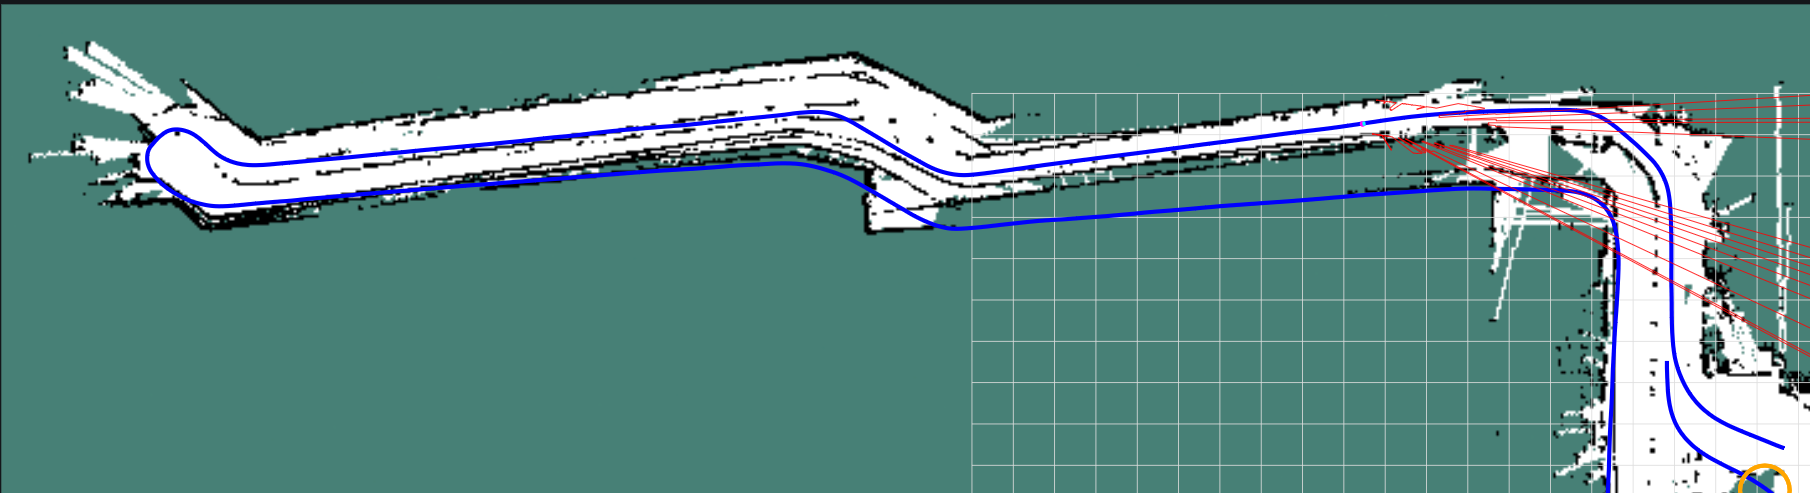
\includegraphics[width=\linewidth]{../konten/map_salah.png}
% 	\caption{Occupancy grid map generated using wheels and IMU only.}
% 	\label{fig:map_hw_odom}
% \end{figure}
% Figures~\ref{fig:map_hw_odom} and~\ref{fig:map_extended_rtabmap} compare the results between wheels and IMU and the Extended RTAB-Map. In these maps, the blue line indicates the ground-truth trajectory.

% \begin{figure}[H]
% 	\centering
% 	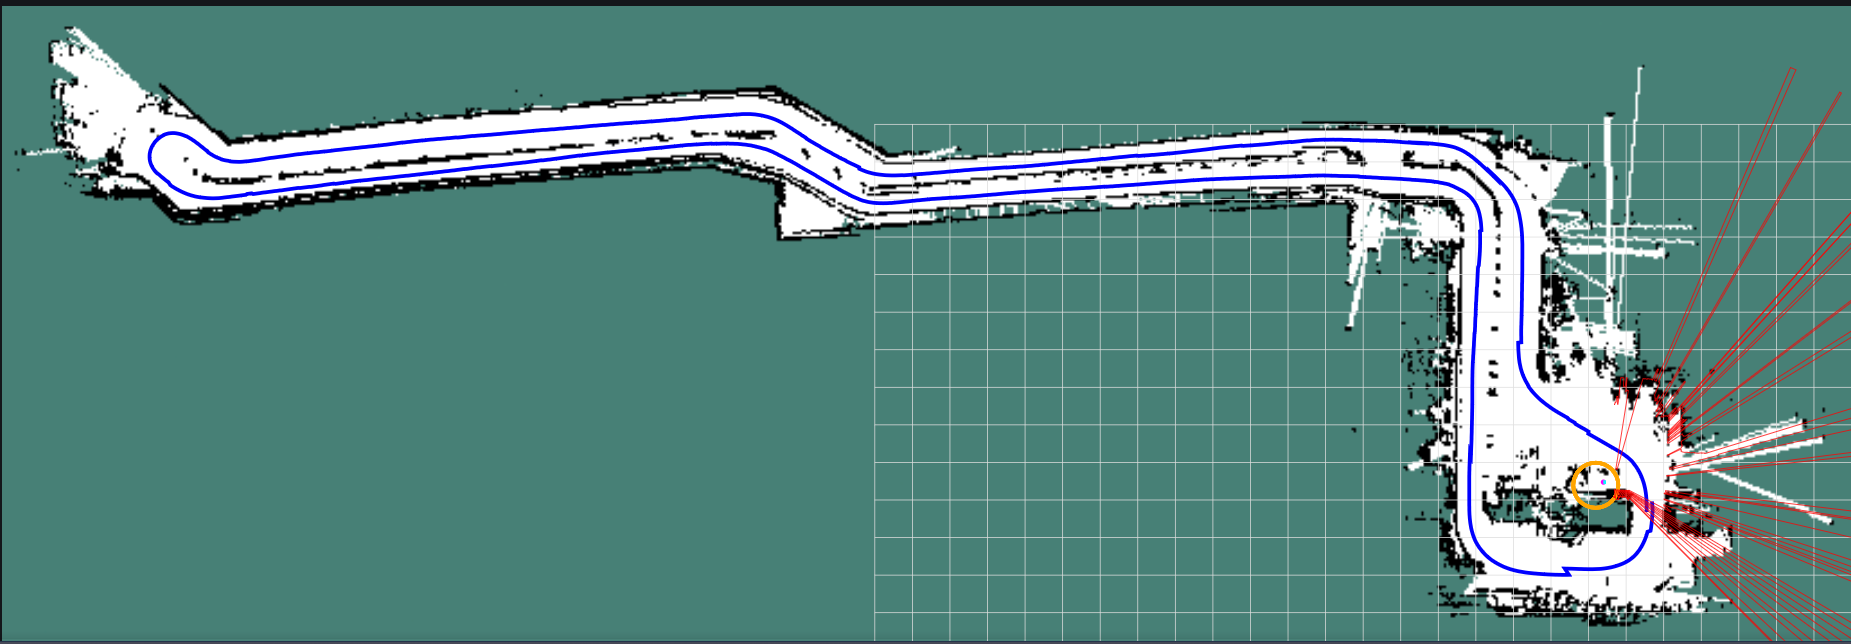
\includegraphics[width=\linewidth]{../konten/map_benar.png}
% 	\caption{Occupancy grid map generated using the Extended RTAB-Map.}
% 	\label{fig:map_extended_rtabmap}
% \end{figure}

% Figures~\ref{fig:map_hw_odom} and~\ref{fig:map_extended_rtabmap} clearly illustrate the difference between the two methods. The map produced by wheels and IMU deviates substantially from the ground truth, exhibiting distorted features due to drift accumulation. In contrast, the map generated by the Extended RTAB-Map aligns closely with the ground truth trajectory, confirming the effectiveness of the proposed approach in enhancing pose estimation accuracy.

\par
Another effective way to visualize the improvement in pose estimation accuracy is through the occupancy grid maps generated by RTAB-Map. The occupancy grid map reflects how well the estimated poses align spatially, providing a visual indicator of mapping consistency. Figure~\ref{fig:map_hw_odom} presents the occupancy grid map produced using wheels and IMU odometry only.

\begin{figure}[H]
\centering
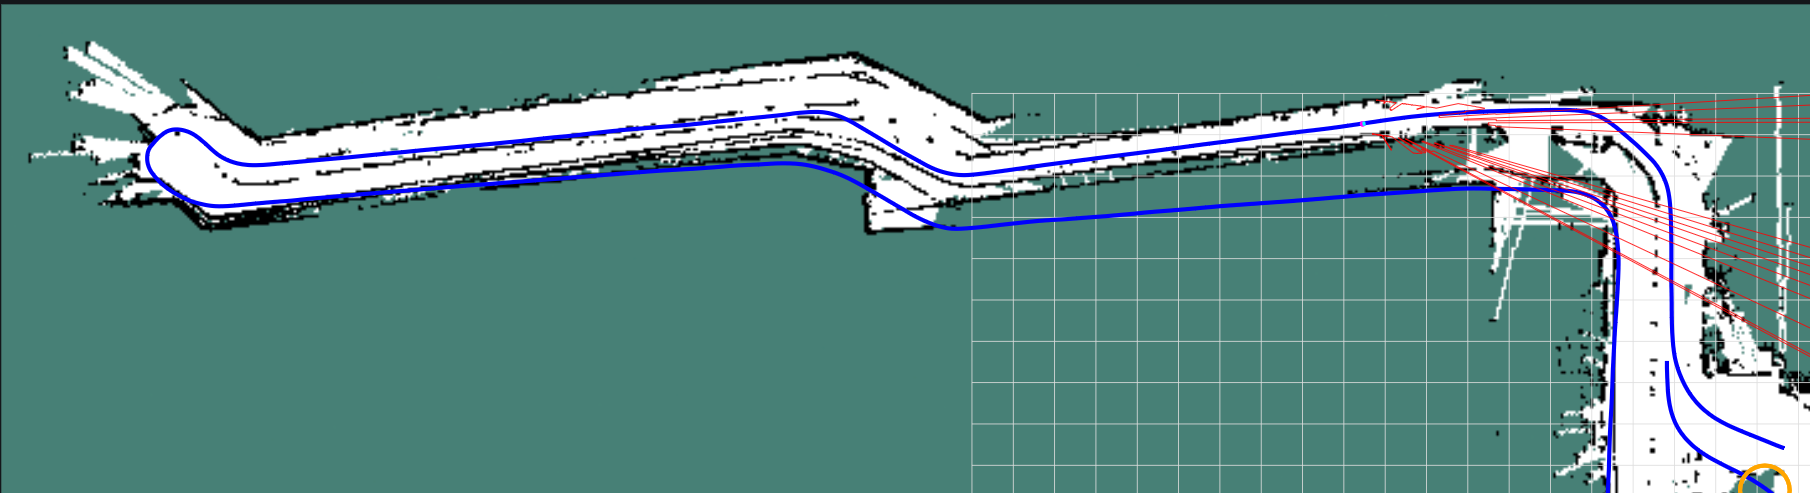
\includegraphics[width=\linewidth]{../konten/map_salah.png}
\caption{Occupancy grid map generated using wheels and IMU odometry only.}
\label{fig:map_hw_odom}
\end{figure}

\par
Figures~\ref{fig:map_hw_odom} and~\ref{fig:map_extended_rtabmap} compare the results obtained from the wheels-IMU odometry and the proposed Extended RTAB-Map method. In both figures, the blue line represents the ground-truth trajectory used for evaluation.

\begin{figure}[H]
\centering
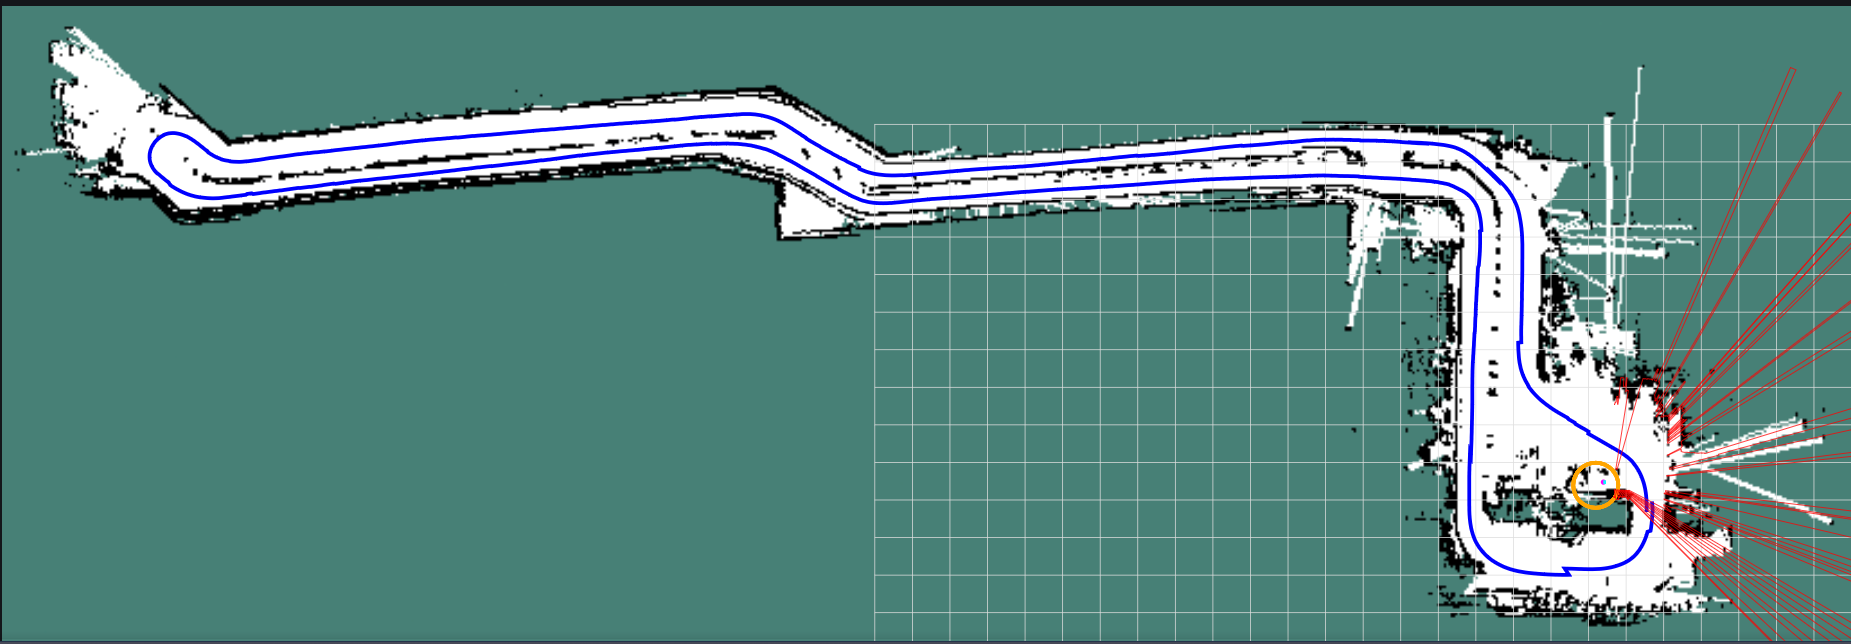
\includegraphics[width=\linewidth]{../konten/map_benar.png}
\caption{Occupancy grid map generated using the Extended RTAB-Map method.}
\label{fig:map_extended_rtabmap}
\end{figure}

\par
The difference between the two maps is clearly observable. The map generated using only wheel and IMU odometry shows significant drift and deformation, leading to misaligned and distorted features. In contrast, the map produced by the Extended RTAB-Map aligns closely with the ground truth trajectory, exhibiting consistent geometry and improved global structure. This confirms the effectiveness of the proposed approach in enhancing pose estimation accuracy and map consistency.

\subsection{Update Rate: Default RTAB-Map vs. Extended RTAB-Map}
The second experiment analyzed the update rate of the pose estimation between the default RTAB-Map and the Extended RTAB-Map. The measurement was conducted using the ROS topic statistics API, which computes the average publishing frequency of the pose topic. The results are shown in Table~\ref{tab:update_rate}.

\begin{table}[H]
	\centering
	\caption{Update Rate Comparison Between Default and Extended RTAB-Map}
	\label{tab:update_rate}
	\begin{tabular}{|c|c|c|}
		\hline
		\textbf{Lap-} & \textbf{RTAB-Map (Hz)} & \textbf{Extended RTAB-Map (Hz)}  \\ \hline
		1 & 1.003 & 50.029 \\ \hline
		2 & 1.002 & 50.006 \\ \hline
		3 & 1.223 & 49.999 \\ \hline
		4 & 1.056 & 49.999 \\ \hline
		5 & 1.332 & 49.998 \\ \hline
		\textbf{Average} & 1.123 & 50.006 \\ \hline
	\end{tabular}
\end{table}

In Table~\ref{tab:update_rate}, RTAB-Map (Hz) represents the average frequency of the default RTAB-Map, and Extended RTAB-Map (Hz) represents the frequency achieved by the proposed system. The average update rate increased from 1.123~Hz to 50.006~Hz, a nearly fiftyfold improvement. This demonstrates that integrating wheels and IMU through the proposed skip connection and Kalman fusion significantly enhances temporal resolution, making real-time pose updates possible without requiring GPU acceleration.

\subsection{Reduced Fast-SCNN Result}
The third experiment evaluated the performance of the proposed Reduced Fast-SCNN model. A custom dataset of 797 labeled images with a resolution of 640$\times$360$\times$3 was developed specifically for this task. The dataset was not divided into training and validation subsets because it represents a complete and absolute sample of the target environment. The model was trained using the Adam optimizer with a learning rate of 0.0001, a batch size of 4, and 100~epochs. A sample of the dataset is shown in Fig.~\ref{fig:dataset_sample}.

\begin{figure}[H]
	\centering
	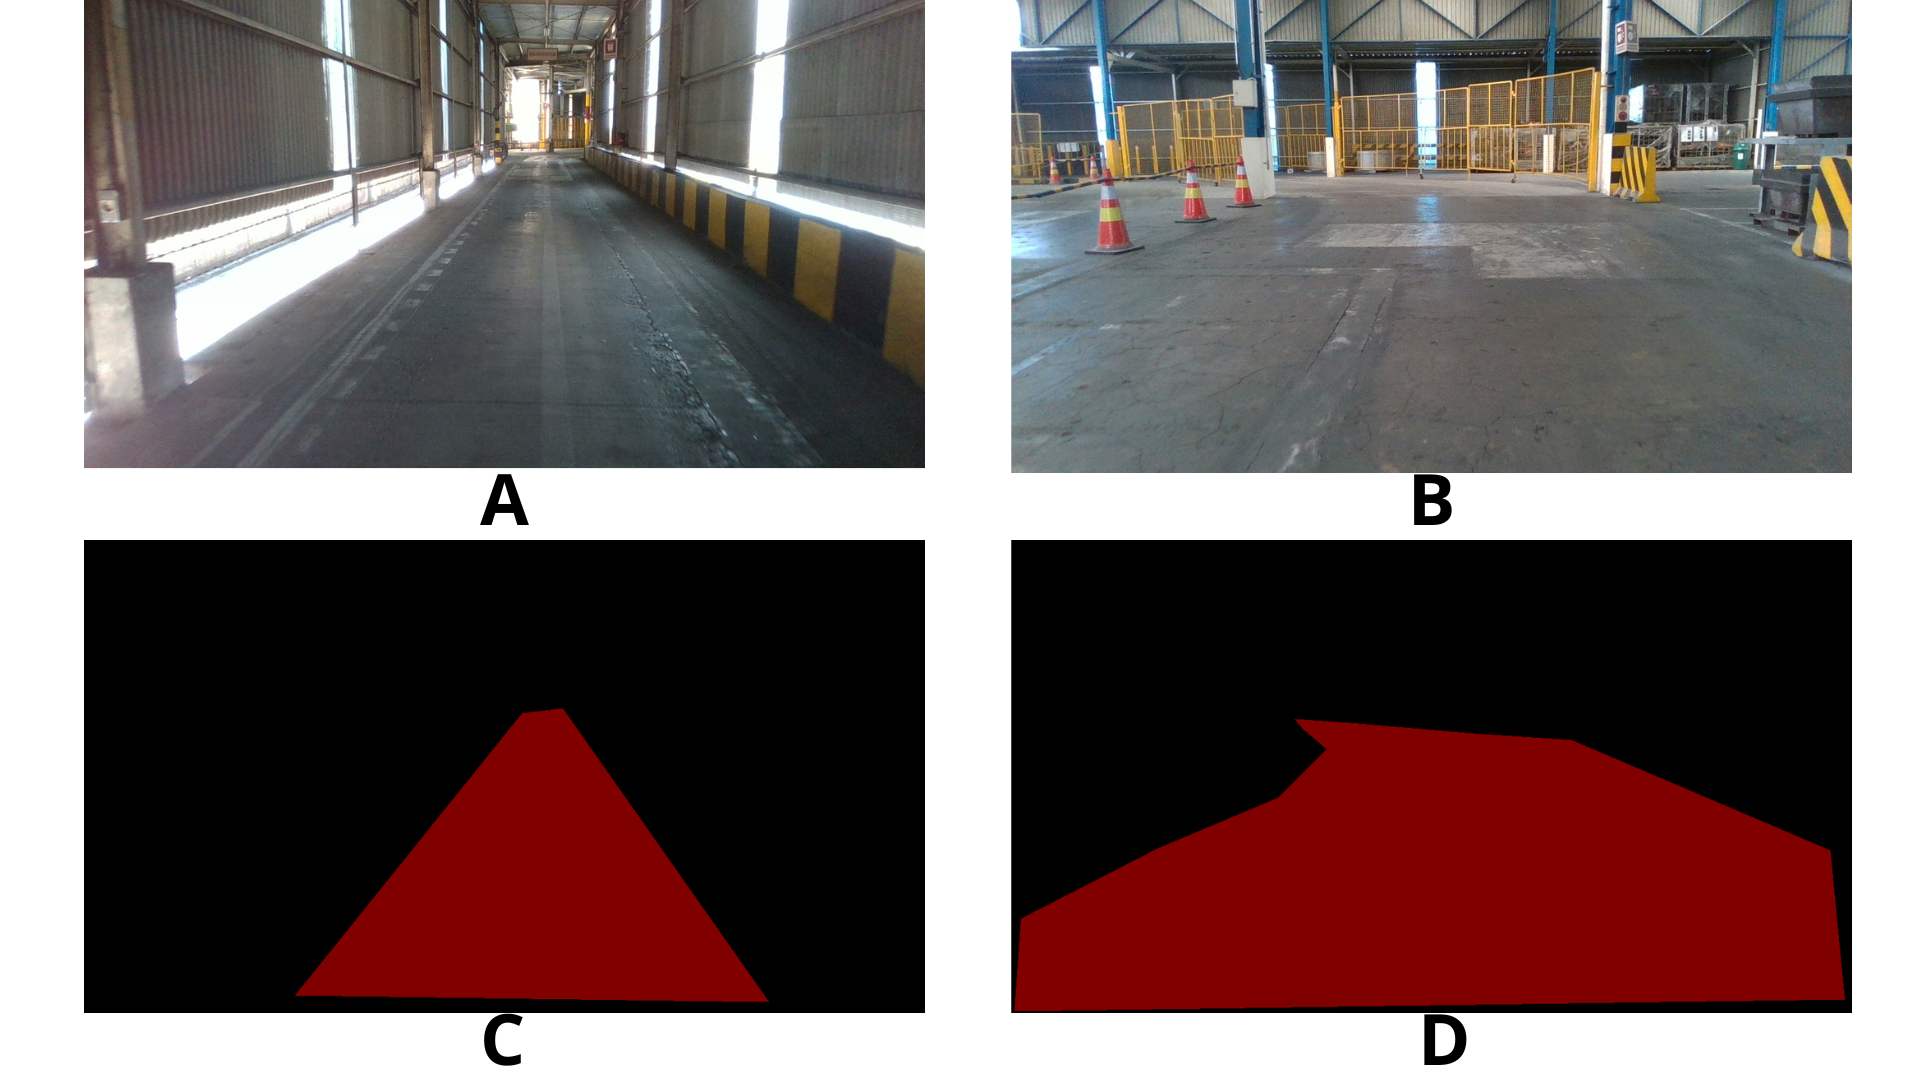
\includegraphics[width=\linewidth]{../konten/dataset_ist.png}
	\caption{Samples from the custom dataset used for training the Reduced Fast-SCNN.}
	\label{fig:dataset_sample}
\end{figure}

In Fig.~\ref{fig:dataset_sample}, images A and B represent RGB inputs from the onboard camera, while images C and D show the corresponding segmentation masks. The segmentation results contain two classes: lane and non-lane regions. The lane pixels are marked in red, while the background is represented in black.

\par
After training, the model was converted into the ONNX format for deployment on CPU hardware. Inference was performed using the ONNX Runtime, which provided approximately a twofold increase in processing speed compared to the native PyTorch implementation \cite{ref_onnx}. Figure~\ref{fig:roi_lane_detection} shows preliminary results of lane detection using the Reduced Fast-SCNN.

\begin{figure}[H]
	\centering
	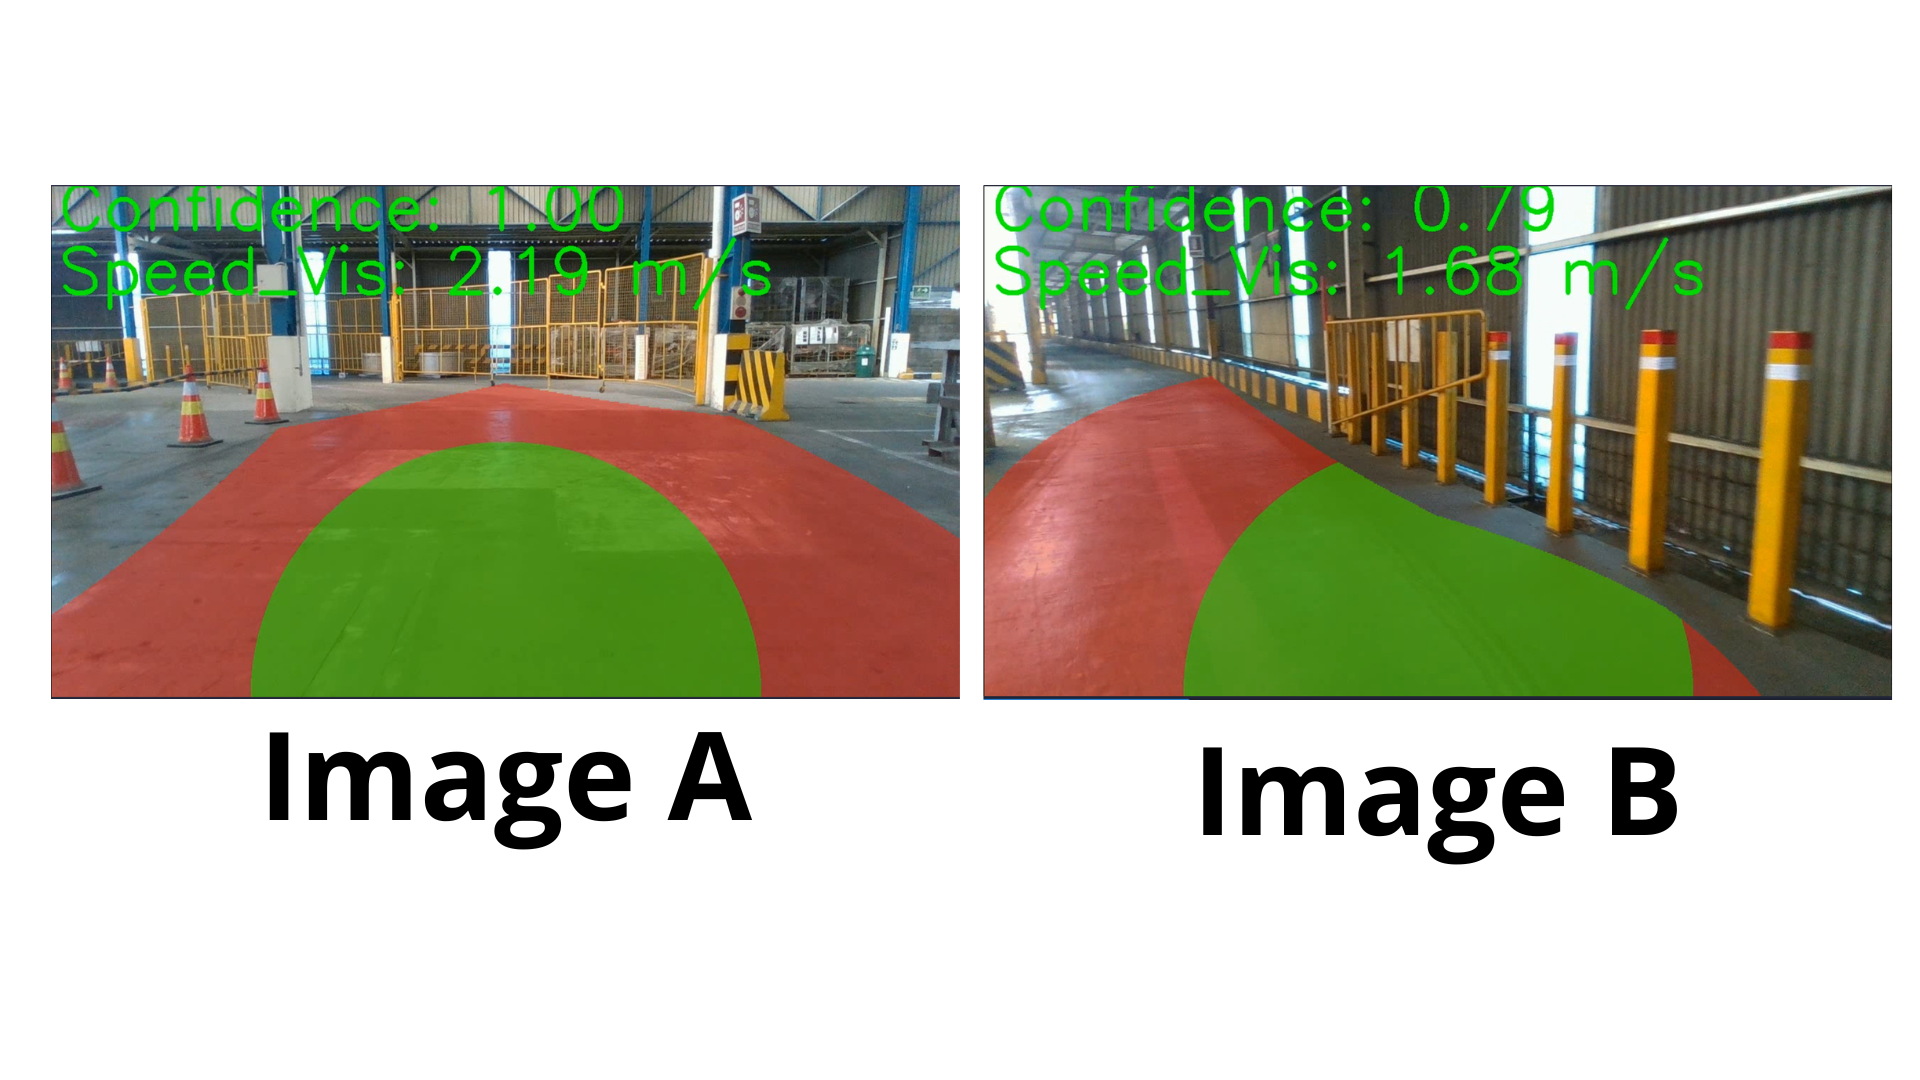
\includegraphics[width=\linewidth]{../konten/pre_res.png}
	\caption{Preliminary lane detection results using the Reduced Fast-SCNN.}
	\label{fig:roi_lane_detection}
\end{figure}

In Fig.~\ref{fig:roi_lane_detection}, the red mask indicates the detected lane area, while the green region represents the region of interest (ROI) used to calculate the confidence level. Image~A shows a full straight lane where the ROI is completely filled, while Image~B shows a turning condition with a truncated ROI, resulting in lower confidence.

\par
The final inference results are displayed in Fig.~\ref{fig:lane_detection_result}.

\begin{figure}[H]
	\centering
	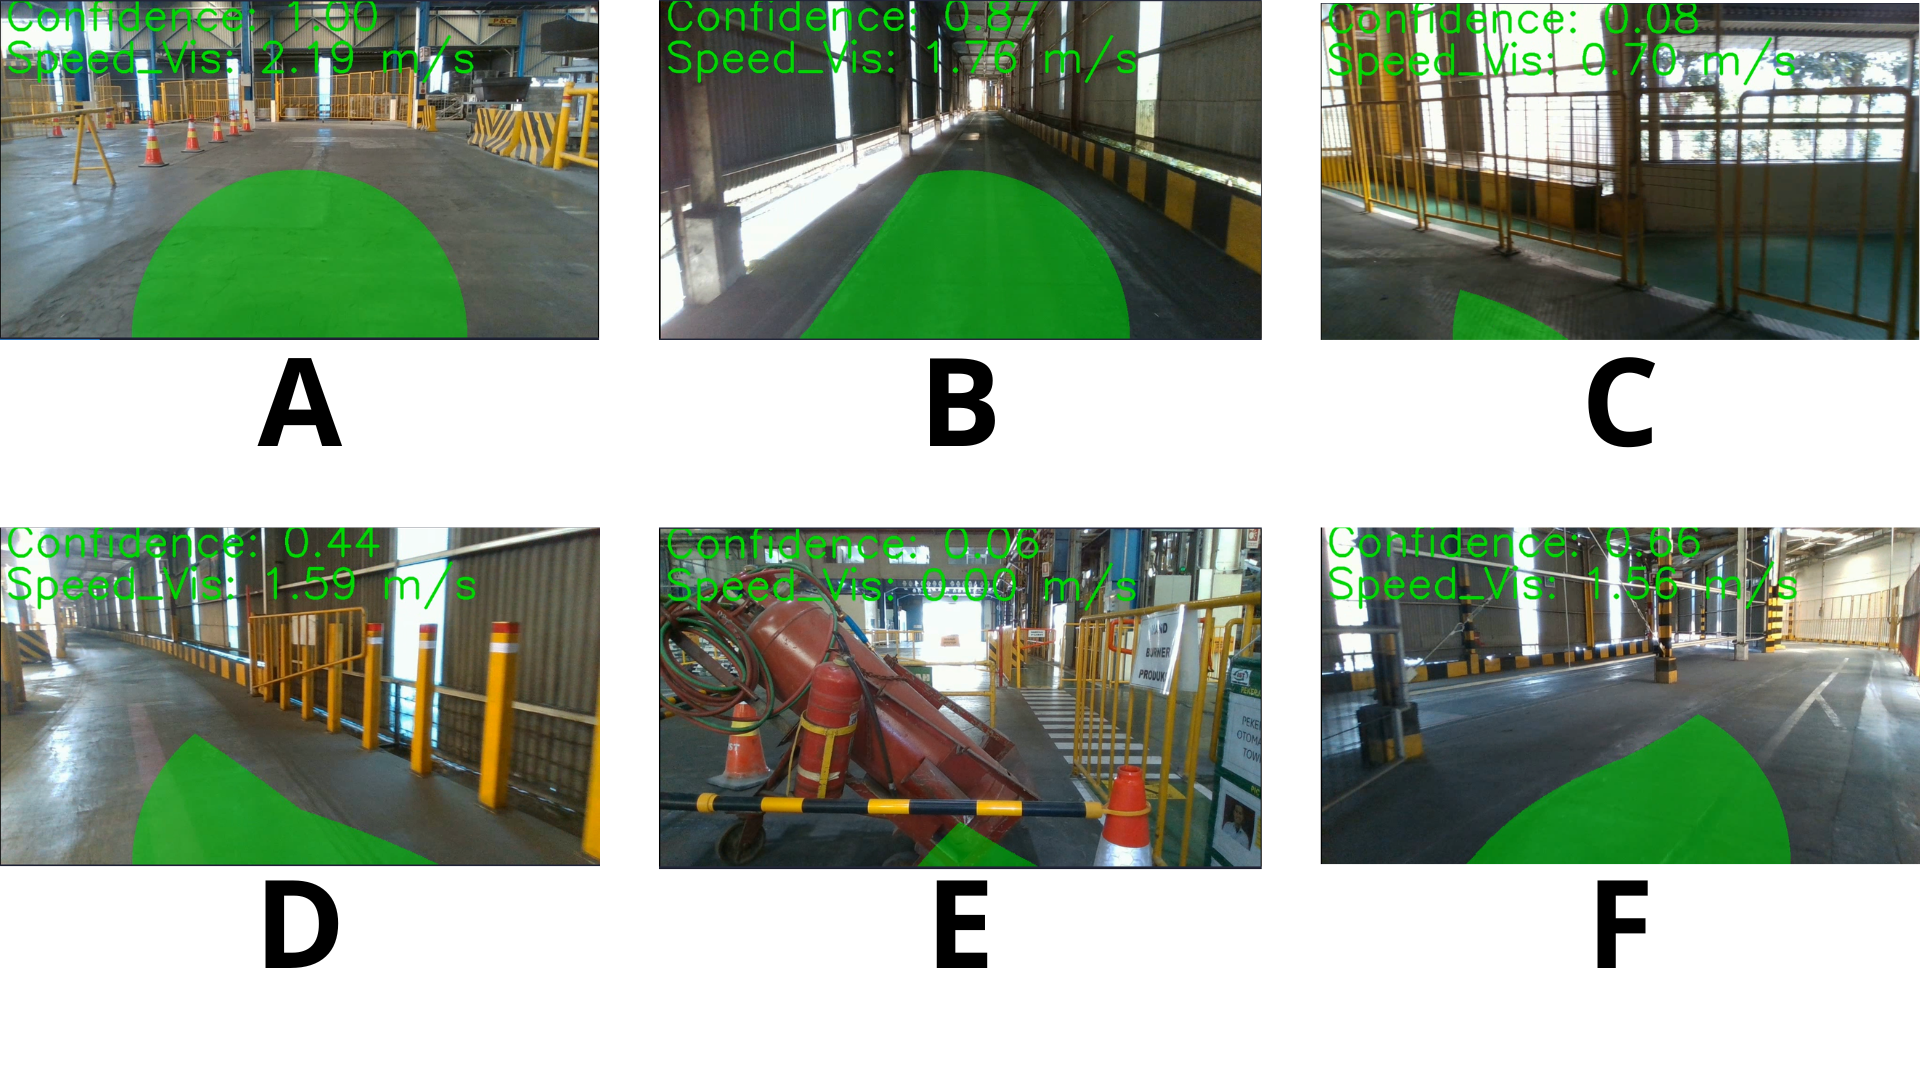
\includegraphics[width=\linewidth]{../konten/bnr_satu.png}
	\caption{Lane detection and velocity control results using the Reduced Fast-SCNN.}
	\label{fig:lane_detection_result}
\end{figure}

Figure~\ref{fig:lane_detection_result} illustrates various driving scenarios. In Image~A, the vehicle is in a full straight lane with an output velocity of 2.2~m/s. Image~B depicts a narrow straight lane with a slightly reduced speed of 1.76~m/s. In Image~C, the vehicle navigates a sharp turn while approaching a fence, resulting in a velocity of 0.70~m/s. Image~D shows a left turn in a narrow area, where the velocity is 1.59~m/s. In Image~E, the vehicle encounters an obstacle directly in front, stopping completely at 0.00~m/s. Finally, Image~F depicts a right turn in a narrow area with a speed of 1.56~m/s. These results demonstrate the effectiveness of the Reduced Fast-SCNN in adjusting the vehicle’s speed based on lane confidence and environmental conditions.

\subsection{Original Fast-SCNN vs. Reduced Fast-SCNN Inference Time}
The final experiment compared the inference time between the original Fast-SCNN and the proposed Reduced Fast-SCNN models. Both were tested on the same hardware platform (2.40 Ghz quadcore CPU , 16~GB RAM, without dedicated GPU). The same test images with a resolution of 640$\times$360$\times$3 were used for consistency. The results are summarized in Table~\ref{tab:lane_detection_inference_time}.

\begin{table}[H]
	\centering
	\caption{Comparison of Inference Time Between Original and Reduced Fast-SCNN}
	\label{tab:lane_detection_inference_time}
	\begin{tabular}{|c|c|c|}
		\hline
		\textbf{Frame Number} & \textbf{Fast-SCNN (ms)} & \textbf{Reduced Fast-SCNN (ms)} \\ \hline
		1 & 22.4 & 7.2 \\ \hline
		2 & 29.3 & 7.7 \\ \hline
		3 & 34.2 & 7.8 \\ \hline
		4 & 39.2 & 7.7 \\ \hline
		5 & 23.8 & 7.4 \\ \hline
		6 & 28.1 & 8.0 \\ \hline
		\textbf{Average} & 29.5 & 7.63 \\ \hline
	\end{tabular}
\end{table}

Table~\ref{tab:lane_detection_inference_time} clearly indicates that the Reduced Fast-SCNN significantly outperforms the original version in terms of speed. The average inference time of the original Fast-SCNN is 29.5~ms per frame, while the Reduced Fast-SCNN achieves an average of 7.63~ms. This improvement corresponds to a nearly 3.9$\times$ reduction in computation time. The results confirm that the proposed architecture is capable of real-time lane detection using CPU-only hardware, making it well suited for industrial autonomous vehicle applications where computational resources are limited.

% =========================================================================================================

\section{Future Development}
There are two primary avenues to improve the local navigation system. The first is to increase robustness in lane detection. This can be achieved by incorporating temporal modeling, for example by using gated recurrent units (GRUs) \cite{ref_gru} to exploit inter-frame dependencies and reduce flicker in the segmentation output. The second direction is to perform velocity and steering control using machine learning. In this approach, control commands can be learned by leveraging the outputs of the lane detection module together with the fused pose estimation, enabling adaptive policies that respond to confidence and environmental context.

\section{Conclusion} 
By utilizing and extending RTAB-Map as the primary algorithm for vehicle pose estimation, we achieve centimeter-level accuracy (error $<5$~cm). This is enabled by introducing a skip connection from wheels and IMU to the pose fusion stage. During fusion, a Kalman Filter combines the corrected pose from RTAB-Map with the odometry-based state, yielding smooth and accurate estimates. The final fused pose attains a 50~Hz update rate on 2.40 Ghz quadcore CPU with 16 GB RAM.

\par
On the perception side, reducing convolutional channels and replacing pyramid pooling with average pooling yields a lightweight, fast segmentation network that runs on CPU alone with sub-10~ms inference. The proposed Reduced Fast-SCNN attains an average inference time of 7.63~ms on the same hardware platform.

\section{Acknowledgment}
This research was supported by Indonesia Smelting Technology (IST), Manufaktur Robot Industri (MRI), and ITS Robotics. The authors would like to thank the teams from IST and MRI for their assistance and collaboration, and the ITS Robotics team for their continued support. Finally, we extend our thanks to ChatGPT and GitHub Copilot for writing support during manuscript preparation.


% Menamcement of realsensepilkan daftar pustaka dengan format IEEE
\bibliographystyle{IEEEtranN}
\bibliography{../ubah/pustaka.bib}

% Menyeimbangkan bagian akhir di kedua kolom
% \balance


\end{document}
